\documentclass[UTF8]{ctexart}

\usepackage{listings}
\usepackage{color,xcolor} 
\usepackage{colortbl}
\usepackage{graphicx}
\usepackage{booktabs} %绘制表格
\usepackage{caption2} %标题居中
\usepackage{geometry}
\usepackage{array}
\usepackage{amsmath}
\usepackage{subfigure} 
\usepackage{longtable}
\usepackage{abstract}
\usepackage{multirow}
\usepackage{enumerate}
\usepackage{float}

%伪代码
\usepackage{algorithm}
\usepackage{algpseudocode}
\usepackage{amsmath}
\renewcommand{\algorithmicrequire}{\textbf{输入:}}  % Use Input in the format of Algorithm
\renewcommand{\algorithmicensure}{\textbf{过程:}} % Use Output in the format of Algorithm


%附录代码
\usepackage{listings}
\usepackage{xcolor}
\lstset{
    numbers=left, 
    numberstyle= \tiny, 
    keywordstyle= \color{ blue!70},
    commentstyle= \color{red!50!green!50!blue!50}, 
    frame=shadowbox, % 阴影效果
    rulesepcolor= \color{ red!20!green!20!blue!20} ,
    escapeinside=``, % 英文分号中可写入中文
    xleftmargin=2em,xrightmargin=2em, aboveskip=1em,
    framexleftmargin=2em
} 

\pagestyle{plain} %页眉消失

\geometry{a4paper,left=2.5cm,right=2.5cm,top=2.5cm,bottom=2.5cm}%设置页面尺寸
\lstset{
		numbers=left, %设置行号位置
		numberstyle=\tiny, %设置行号大小	
		keywordstyle=\color{blue}, %设置关键字颜色
		commentstyle=\color[cmyk]{1,0,1,0}, %设置注释颜色
		escapeinside=``, %逃逸字符(1左面的键),用于显示中文
		breaklines, %自动折行
		extendedchars=false, %解决代码跨页时,章节标题,页眉等汉字不显示的问题
		xleftmargin=1em,xrightmargin=1em, aboveskip=1em, %设置边距
		tabsize=4, %设置tab空格数
		showspaces=false %不显示空格
	}


		% \begin{figure}[!htbp]\centering
		% \includegraphics[width=1\textwidth]{img} % 图片相对位置
		% \label{fig:figure 0} % 图片标签
		% \end{figure}


\title{基于\textbf{XXXXX}XX的葡萄酒评价}
\date{August 24, 2022}

\begin{document}
\maketitle{}
\renewcommand{\abstractname}{\Large 摘要\\}
\begin{abstract}
	\normalsize
	葡萄酒备受大部分人的热爱,质量较好的葡萄酒往往带来更好的感官体验。葡萄酒的评价有着不同的指标,但其好坏却主要来自于评酒师的个人主观评价,所以会导致评价结果的差异性和不够客观性,存在着不同大众的口味喜爱偏差。本文为了解决该问题,通过探索酿酒葡萄对葡萄酒质量的影响,通过建立模型的方式更合理的对酿酒葡萄质量分类,以及如何依赖不同的酿酒葡萄和葡萄酒之间的关系来客观的给出葡萄酒评价结果,通过客观修正的数据建立了数学模型,以客观的方式来给出葡萄酒的评价。

	针对问题一,由于数据较多,且分布不均的原因,首先通过对数据的筛选处理,发现两组对红葡萄酒和白葡萄酒的打分情况是两两相互比较和配对进行K-S检验判断数据是否符合正态分布,再对样本T检验进行显著性差异判断,通过方差齐性检验来假设检验,最后依据显著性差异水平来判断打分组别的稳定性和可靠性。

	针对问题二,需要对酿酒葡萄进行分类,需要考虑到所酿葡萄酒的好坏。由于评酒员的打分存在主观性的干扰,我们将打分数据重新加权处理求和,得到一份较为中肯的综合评价结果。对酿酒葡萄和葡萄酒理化指标进行标准化处理,去除机值,后利用主成分分析对酿酒葡萄和葡萄酒理化指标提取主成分。将酿酒葡萄的数据和葡萄酒理化指标数据进行关联,采用改进的K-means++分类模型,通过对主成分聚类分析将葡萄酒质量分为六大类,由于部分葡萄酒得分评价数值较低,以此为下限进行分类,借鉴罗伯特帕克葡萄酒评分体系依据酿酒葡萄和葡萄酒的相关性,以酿酒葡萄的理化指标含量和分布来进行排名,分出酿酒葡萄的等级和优劣。

	针对问题三,探求酿酒葡萄和葡萄酒的理化指标之间的关系。首先对数据进行筛选处理出关键数据,剔除部分多余数据。提取葡萄酒某指标以及对应的酿酒葡萄理化指标进行相关性分析,通过perason系数和显著性水平来判断其相关性的强弱。后获取到相关性较强的理化指标数据进行共线性诊断后,进行德宾沃森残差分析后通过多元回归的方法来进行拟合,以R方的值来判断拟合的契合度高低,以高的模型数据为准得到葡萄酒和对应酿酒葡萄理化指标之间的系数,建立其函数关系。

	针对问题四,借鉴问题二中使用到的主成分分析法先对酿酒葡萄的理化指标进行分类,提取到八大类主成分,分析各主成分中相关较高的酿酒葡萄和葡萄酒的理化指标,从而得到对葡萄酒质量贡献较大的因素指标。对评分数据进行加权求和、去极值处理后。以评分标准数据作为因变量,酿酒葡萄理化指标主成分作为自变量来进行回归分析,得出回归的评分表。通过误差分析来分析以理化指标得出的评价和已给出的评价之间的误差,来判断是否能以葡萄酒和酿酒葡萄的理化指标作为葡萄酒质量的评价标准。

	\textbf{关键字}:K-S检验  聚类分析  主成分分析 K-means++分类模型 相关性分析 多元回归	Perason系数

\end{abstract}


\section{问题背景与重述}
\subsection{问题背景}
葡萄酒是当今世界上最畅销的酒类之一,在各种场合都有葡萄酒的身影。然而葡萄酒的酿造是取决于多种因素,各种因素的叠加会导致葡萄酒的品质差异明显。在不同的原材料已经酿制方法的差别下葡萄酒会继续细分,例如红葡萄酒和白葡萄酒等。对各种葡萄酒的鉴别是必不可少的一个步骤,而采用人工品尝打分和采用仪器进行理化指标的检验已成为最为科学的鉴别方法。最后经过安全检查、筛选分级的葡萄酒方可上市成为饮用酒。
\subsection{题目所给信息及参数}
此次比赛是根据10位品酒员为27款红酒和28款白葡萄酒的打分,以及上述葡萄酒的指标情况和芳香物质为基础进行数学分析和建模,并探讨品酒员的打分是否合理以及论证是否科学分级。红葡萄酒和白葡萄酒的市场在国际上的价值非常之高,葡萄酒依旧是未来的主力酒类,对此分析依旧存在价值。现在根据三个数据文件,并对三个数据进行分析处理后描述统计,完成数学建模和预测。

数据一:葡萄酒品尝评分表;数据二:指标总表;数据三:芳香物质。
\subsection{所需解决的问题}
1. 根据附件所提供的两组品酒员对27款红葡萄酒和28款白葡萄酒的打分判断两组结果是否有显著性差异,并判断哪一组的更加可信。

2. 根据酿酒葡萄的理化指标和葡萄酒的质量,使用无监督方法计算相似度,通过相似度进行分级。

3. 分析酿酒葡萄和葡萄酒的理化指标之间是否具有相关性,以及其之间具有什么样的联系。

4. 通过主成分分析对数据进行降维,得到贡献值大的特征进行表示,建立其函数关系,根据建立的函数进行预测,将预测结果与评分标准进行误差分析,判断建立的模型是否合理。


\section{问题分析}
针对不同的国家,地区和相对应的医疗水平进行对应的数据指标分析。主要分析感染率,病人接触率,治愈率,以及传染期接触数。
模型构建还需要考虑到新冠肺炎的无症状感染者这一特殊的情况,根据这些指标进行相轨线分析,合理的进行疫情的分析和未来疫情走向以及各地区、国家的防疫政策研究。
\subsection{问题一的分析}
第一,根据附件1中给出两组品酒员的打分情况判断两组的打分是否有显著性差异。对于此问题,分析附件一所提供的数据,
研究发现两组对红葡萄酒和白葡萄酒的打分情况是两两相互比较和配对,适合于先进行单样本K-S检验判断数据是否符合正态分布,
再进行两配对样本T检验进行显著性差异判断的办法。

第二,判断两组品酒员的打分情况哪一组更加可信。对于此问题,分析两组品酒员的打分情况,检验两组中打分的更稳定的一方,
越稳定的分数即代表品酒员偏好更少,更加可信。提取两组品酒员对于白葡萄酒和红葡萄酒的分数的标准差,根据标准差的大小进行可信性的判断。

\subsection{问题二的分析}
基于改进的K-means++\cite{arthur2006k}进行分类模型,为了降低数据数,首先对红、白葡萄和葡萄酒理化指标采用主成分分析法提取出主成分,但是经过Bartlett球形度检验\cite{arsham2011bartlett}等发现不适合进行主成分分析,进行标准化处理,去除极值,使评价分数更加客观,然后借鉴Robert Parker葡萄酒评分体系\cite{hommerberg2011persuasiveness},对这些主成分聚类分析得出6种聚类并依据判别标准(聚类后葡萄酒样本的平均值),最终确定红、白葡萄的分级。

\subsection{问题三的分析}
首先要参照附件所给的数据来进行分析酿酒葡萄和葡萄酒之间的相关性,附件的信息内容过多,需要进行合理的过滤和筛选数据,
但要尽可能保证其数据的完整性和真实性。我们采取相关性分析,依据相关性皮尔森系数来判断葡萄酒的数据和酿酒葡萄的理化指标之间的相关性显著程度。

在进行了相关性分析后,可以确定下一些具有显著相关的数据流,要进一步解决其葡萄酒某指标与该些理化指标的关系,
则要进行其关系的拟合,从而得出实质性的结论来判断酿酒葡萄和葡萄酒之间的关系,以及其关系的可靠性。
\subsection{问题四的分析}


\section{符号说明}
\begin{table}[!htbp]
	\begin{center}
		\begin{tabular}{c|l}
			\toprule[2pt]
			\rowcolor[gray]{0.8}

			\multicolumn{1}{m{8em}}{\centering 符号} & \multicolumn{1}{m{30em}}{\centering 基本说明}        \\

			%直接用合并单元格的方法来实现自定义列宽的同时,使文字居中对齐

			\midrule[1.3pt]
			$S(t)$                                   & 表示t时刻\ 易感人群\ 的总人数                        \\
			%		$E(t)$ & 表示t时刻\ 潜伏期人数\ 占总人数的比例 \\   
			$I(t)$                                   & 表示t时刻\ 感染人数\ 的总人数                        \\
			$R(t)$                                   & 表示t时刻\ 退出者(治愈+死亡)的总人数               \\
			$Y(t)$                                   & 表示t时刻\ 疑似者(实际被感染+实际未被感染)的总人数 \\
			$N(t)$                                   & 表示t时刻\ 所有未隔离患者\ 的总人数                  \\
			$\kappa$                                 & 疑似人群中被确定未感染人数占疑似人群总数的比例       \\
			$\lambda$                                & 隔离者被确诊人数占隔离者总人数的比例                 \\
			$\theta$                                 & 被隔离的人数占未隔离总人数的比例                     \\
			$\omega$                                 & 被确诊且隔离人数占未隔离总人数的比例                 \\
			$\rho$                                   & 感染者平均每天对任何状态的人的接触率                 \\
			$\xi$                                    & 退出率(死亡率+治愈率)                              \\
			\bottomrule[2pt]
		\end{tabular}
	\end{center}
\end{table}
\section{模型假设}

% 模型假设部分
\begin{itemize}
	\item [\bf{1)}]\bf{考虑到目前已处于疫情控制阶段,且人们自我隔离意识较好,不妨设每个病人的有效日接触率为定值}
	\item [2)]\bf{所有人口都为易感染者,不考虑个别免疫体质}
	\item [3)]\bf{疑似病例一旦确诊即被隔离,不会再传播给他人}
	\item [4)]\bf{隔离人群中一旦被确定未感染,则立刻结束隔离,即恢复易感者身份}
	\item [5)]\bf{在考虑隔离者与未隔离者时将确诊感染者和潜伏期患者都定义为感染者}

\end{itemize}



\section{模型建立与求解}
\subsection{问题一的求解}
问题一分析两组评酒员的评价结果有无显著性差异,并判断两组结果哪一组更加可信。采用三个步骤完成分析,步骤如下:


\subsubsection{数据的预处理}
因为数据较大,指标较多,所以我们对各项分数相加得到总分,接着取平均值进行比较。

均值计算如下:
\begin{equation}
	x = \sum_{x_{mn}}^{10}(m = 1,2,3,,,10  n = 1,2,3,,,10)
\end{equation}

\subsubsection{各葡萄酒样本评分数据概率分布的确定}
对两组品酒员差异性评价的假设检验一般要求数据符合正态分布,因为两配对样本T检验的前提要求为数据符合正态分布,才可以使用T检验的数学模型。
利用 SPSS 统计软件中单样本 K-S 检验\cite{young1977proof}, 对数据集两组品酒员分别对红、白葡萄酒品尝得到的四组评价结果进行了正态分布检验。

% \begin{figure}[H]\centering
% 	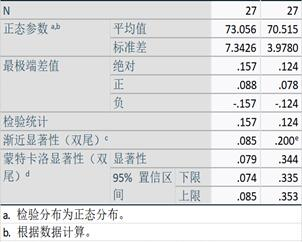
\includegraphics[width=0.45\textwidth]{img/1/red_k_S.png} % 图片相对位置 
% 	\caption{聚类汇总图} % 图片标题 
% 	\label{fig:figure 1} % 图片标签
% \end{figure}

% \begin{figure}[H]\centering
% 	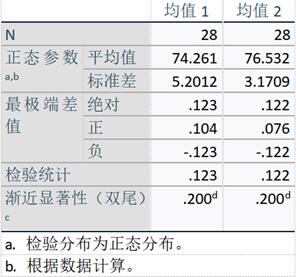
\includegraphics[width=0.45\textwidth]{img/1/white_k_S.png} % 图片相对位置 
% 	\caption{聚类汇总图} % 图片标题 
% 	\label{fig:figure 2} % 图片标签
% \end{figure}

从图1\label{figure 1}和图2\label{figure 2}可以看出两组的双边检验结果。因此可以认为品酒员对葡萄酒的评分服从正态分布。

\subsubsection{两组评价结果的显著性差异评价}
上述检验显示各类葡萄酒得分情况属于正态总体,为了进一步说明品酒员评分的科学性以及两个评分组评分的可信度, 需要检查两组给出的评分是否有显著性差异, 即对数据进行显著性检验。

两配对样本非参数检验一般用于同一研究对象分别给予两种不同处理的效果比较。因为两组品酒员分别对同一样本组进行评分,故两组数据为配对数据。

\begin{equation}
	z_{li} = w_{li}-w_{2i}(i=1,2,,,,n)
\end{equation}

$z_li$来自正态分布,用假设检验的方法,假设$H_{0}:u_1=0$成立;
\[\left\{\begin{array}{llcl}

		\bar{z}=\frac{1}{n}\sum_{i=1}^n(Z_li)         \\

		s_{1}^2=\frac{1}{n-1}\sum_{i=1}^n(z_li-z_1)^2 \\

		t=\frac{\bar{z_1}}{\frac{s_1}{\sqrt{n}}}      \\

		w={\mid t \mid \ge t_{1-\frac{a}{2}}(n-1)}    \\

		% 	% S(t_0)&=&140005\times10^4&\text{人},\\
		% 	% I(t_0)&=&14052 &\text{人},\\
		% 	% R(t_0)&=&130 &\text{人},\\
		% 	% Y(t_0)&=&4562 &\text{人},\\
		% 	% N(t_0)&=&6336 &\text{人},\\
	\end{array} \right.\]

对于统计量t,在给定显著性水平a下,该检验问题的拒绝域是w,若${\mid t \mid \ge t_{1-\frac{a}{2}}(n-1)}$,则拒绝假设反之则接受。

\begin{center}
	\begin{tabular}{||c c c c c c||}
		\hline
		组数 & 样本数 & 平均值 & 标准差 & $T_1$值 & p      \\ [0.5ex]
		\hline
		一   & 27     & 73.056 & 3.9780 & 2.458   & 0.0104 \\
		\hline
		二   & 27     & 70.515 & 7.3426 & 2.458   & 0.0104 \\
		\hline
	\end{tabular}
\end{center}

上表给出了两组红葡萄酒评分均值的t检验结果,通过查表当x =0.05, n=27时, $t_{1-\frac{a}{2}}(n-1)=2.0555<2.491$
且方差齐性检验的$p$值为0.0104<0.05,
所以拒绝原假设,对于红葡萄酒的评价,两组评酒员的评价结果有显著性差异。
因为第二组评酒员对红葡萄酒样品评分的标准差大于第一组的,第二组各评酒员得评分差异小,稳定性高,比较可信。

对于白葡萄酒采用同样的方法,得到了如下的表格:
\begin{center}
	\begin{tabular}{||c c c c c c||}
		\hline
		组数 & 样本数 & 平均值 & 标准差 & $T_1$值 & p       \\ [0.5ex]
		\hline
		一   & 28     & 74.261 & 5.2012 & -2.184  & 0.01892 \\
		\hline
		二   & 28     & 76.532 & 3.1709 & -2.184  & 0.01892 \\
		\hline
	\end{tabular}
\end{center}

上表给出了两组红葡萄酒评分均值的$t$检验结果,通过查表当$x=0.05$, $n=28$时, $t_{1-\frac{a}{2}}(n-1)=2.0555<2.491$且方差齐性检验的$p$值为0. 01892<0.05,所以拒绝原假设,对于白葡萄酒的评价,两组评酒员的评价结果有显著性差异。因为第一组评酒员对红葡萄酒样品评分的标准差大于第二组,第二组各评酒员得评分差异小,稳定性高,比较可信。

综上分别对两组葡萄酒进行T检验\cite{de2013using},在显著性水平为0.05时,得出两组评酒员的评价结果有显著性差异,第二组评酒员的评分更可信。


\subsection{问题二的求解}

\subsection{问题三的求解}


%引用
\clearpage
\bibliographystyle{plain}
\bibliography{ref}%ref指向自己创建的ref.bib
% IoU\cite{zheng2020distance}
\clearpage

\section{附录}
\subsection{代码}

\lstset{language=python}
\begin{lstlisting}
	import time
	import numpy as np
	import pandas as pd
	import matplotlib.pyplot as plt

		
\end{lstlisting}

\end{document}
